\section{Experimental Evaluation}
\label{sec:experiments}

We evaluate the fixed procedure in Equation~\ref{eq:fusion} on three Beijing panels, and examine statistical-component transfer on three HDB panels. All reported errors use one consistent result snapshot and the original future observation masks. The method and its application focus were selected retrospectively using these development results. Consequently, the experiments characterize performance on the observed cohorts and do not constitute independent confirmation of the selected method. The same primary definition is retained across the three Beijing panels.

\subsection{Data, Information and Metrics}

\paragraph{Beijing sensor forecasting.}
The Beijing Multi-Site Air Quality dataset contains hourly measurements from 12 stations between March 2013 and February 2017~\citep{uci2017beijing}. We predict PM2.5 and PM10 from eleven numerical station variables and six prefix-selected peer PM channels. All statistical fitting uses the first 7012 hours of each augmented station series. Evaluation origins follow the 60\% temporal boundary, with the current 192-hour context entirely after that boundary. The primary and matched long-history controls use 8192 pre-origin hours. Related measurements use the provider's aligned hourly clock; their availability before the origin is assumed, without a separate publication-delay model.

Natural-outage origins require both PM targets to have been continuously missing for at least six hours. Origins occur at outage ages $6+24k$ hours, with nonoverlapping 24-hour forecast intervals within a station. Each target must have at least twelve observed future values to be scored. The resulting panel contains 45 windows across 12 stations; 32 additional candidate origins lack sufficient observed future labels. This ascertainment can favor events that recover observations sooner. Artificial outages use four complete histories per station, selected at evenly spaced chronological positions, and hide only the last 24 hours of the two targets. The 138-window horizon-96 panel retains original target missingness and requires at least 48 observed future values per target. Table~\ref{tab:data} summarizes these populations and the HDB component study.

\begin{table}[t]
\caption{Evaluation populations. Windows are prediction tasks, and sites within a source are correlated. All panels are developmental. The HDB study evaluates available statistical-component variants, with no recorded result for the exact peer-regression primary.}
\label{tab:data}
\centering\small
\begin{tabular}{llrrr}
\toprule
Source & Panel & Sites & Windows & Horizon (h)\\
\midrule
Beijing & Natural target outage & 12 & 45 & 24\\
Beijing & Artificial target outage & 12 & 48 & 24\\
Beijing & Original missing history & 12 & 138 & 96\\
HDB & Natural availability gap & 18 & 19 & 24\\
HDB & Artificial target outage & 18 & 32 & 24\\
HDB & Native hourly grid & 18 & 32 & 24\\
\bottomrule
\end{tabular}
\end{table}

\paragraph{HDB component-transfer population.}
The second source is Singapore HDB carpark availability~\citep{hdbavailability}. Hourly snapshots cover 1 June--26 July 2025, yielding 1344 time positions and 2005 C-type carpark series. The first 336 hours supply fitting statistics and peer selection; the next 336 hours supply the development cohort. All eighteen prefix-eligible carparks with natural events in that development period are retained. The remaining two 336-hour intervals are unscored. Natural gaps, missing records, stale observations and collection failures are distinguished, with technical failures excluded from the natural-missingness interpretation. A target is accompanied by six prefix-selected peers. Long histories contain the available 349--586 pre-origin hours. The exact Beijing peer-regression method has no recorded HDB evaluation; the Gaussian repair, fixed fusion and native controls permit a narrower component-transfer comparison.

\paragraph{Evaluation metric.}
Let $n_k=\sum_hV_{hk}$ and let $s_k$ be the original-observation prefix scale. We compute
\begin{align}
 \operatorname{MAE}(\widehat Y,Y)&=\frac1K\sum_k\frac1{n_k}
   \sum_{h:V_{hk}=1}\frac{|\widehat Y_{hk}-Y_{hk}|}{s_k},\nonumber\\
 \operatorname{MSE}(\widehat Y,Y)&=\frac1K\sum_k\frac1{n_k}
   \sum_{h:V_{hk}=1}\frac{(\widehat Y_{hk}-Y_{hk})^2}{s_k^2}.
 \label{eq:metrics}
\end{align}
Equation~\ref{eq:metrics} averages targets within a window, then windows within each site, and finally sites with equal weights. Missing future values are never completed to manufacture labels. MAE is primary, and both metrics are retained for every comparison. Relative change is $100(\mathrm{method}/\mathrm{reference}-1)$, so negative values denote lower error. We report paired site directions and leave-one-site-out ranges as descriptive sensitivity analyses, without treating them as confidence intervals or converting repeated development comparisons into significance claims.

\subsection{Comparators and Fitting Budgets}

The frozen backbone is the same 120M-parameter Chronos-2 checkpoint throughout~\citep{ansari2025chronos2}. Native controls retain missing values and use either 192 hours or the available long context. Separate controls retain only the target variables, providing an explicit input-scope comparison. VAR uses the same fitted statistical branch as the primary. Native-plus-VAR controls hold both the history and fusion weight fixed while omitting target repair.

Repair controls include LOCF, linear interpolation, seasonal copying, multivariate KNN, SAITS, TimeMixer++ and MoTM. The neural imputers use two shared 17-variable Beijing fits, each trained on 512 masked prefix windows for 50 epochs, with batch size 16 and seed zero. MoTM retains its released weights and its fixed observed-context adaptation procedure. Short-history comparisons include each target-only repair and the mean/median of the seven repaired predictions plus native prediction. Additional all-variable repairs and statistical regression variants are retained in the supplement. A fixed Gaussian control estimates prefix means and regularized covariance and applies the conditional mean independently at each time. The same long-history and VAR-fusion factors are applied to Gaussian, KNN and ridge repairs.

Two LoRA controls add 1,206,912 parameters to 97 Chronos-2 projections, with rank eight and scaling parameter sixteen. Natural-history and corruption-trained versions share initialization, source labels, update order and 1728 single-task updates, split equally between Beijing and HDB. They use standardized smooth L1 loss with parameter 0.01, AdamW learning rate $10^{-5}$, weight decay 0.01 and gradient-norm limit one. Evaluation uses the final update. These adapted controls have a different training budget from the statistical primary; their stronger results are still retained. Appendix~\ref{app:training} gives the source boundaries and additional implementation details.

\subsection{Main Results on Natural Sensor Outages}

Table~\ref{tab:main} compares fixed methods across all three Beijing panels. On natural outages, \method{} reaches MAE/MSE 0.388053/0.244688. Relative to the long native forecaster, the reductions are 19.96\% and 31.90\%. The matched native-plus-VAR comparison isolates the effect of adding target repair under the same long history and statistical forecast: MAE/MSE decrease from 0.412755/0.263833 by 5.98\%/7.26\%. Against short target-KNN repair with the same VAR fusion, reductions are 2.25\%/7.46\%.

\begin{table}[t]
\caption{Beijing results. Each row has one fixed definition across panels. Long histories contain 8192 hours; unqualified inputs include the available local and peer variables. ``Targets only'' changes the variables supplied to the forecaster. Values are standardized MAE/MSE; lower is better. Bold marks the best value in each displayed column.}
\label{tab:main}
\centering\footnotesize
\setlength{\tabcolsep}{3.3pt}
\begin{tabular}{lrrrrrr}
\toprule
 & \multicolumn{2}{c}{Natural, $H=24$} & \multicolumn{2}{c}{Artificial, $H=24$} & \multicolumn{2}{c}{Original, $H=96$}\\
Method & MAE & MSE & MAE & MSE & MAE & MSE\\
\midrule
Native, 192 h & 0.5302 & 0.4359 & 0.8300 & 1.2501 & 0.8633 & 1.6678 \\
Native, long & 0.4848 & 0.3593 & 0.6665 & 0.8567 & 0.7965 & 1.4456 \\
Native, long, targets only & 0.5351 & 0.4406 & 0.6786 & 1.0608 & \textbf{0.7898} & 1.4165 \\
VAR & 0.4336 & 0.3037 & 0.6628 & 0.8248 & 0.8740 & 1.3634 \\
Native, long + VAR & 0.4128 & 0.2638 & 0.6354 & 0.7795 & 0.8098 & 1.3269 \\
Native, long, targets + VAR & 0.4347 & 0.2914 & 0.6170 & 0.7453 & 0.8052 & \textbf{1.3130} \\
Target KNN, 192 h + VAR & 0.3970 & 0.2644 & 0.6648 & 0.9118 & 0.8342 & 1.4266 \\
Gaussian repair, long & 0.3918 & 0.2524 & 0.6289 & 0.8660 & 0.7966 & 1.4498 \\
Gaussian repair, long + VAR & 0.3882 & 0.2451 & 0.6310 & 0.8110 & 0.8100 & 1.3290 \\
KNN repair, long + VAR & 0.3887 & \textbf{0.2441} & 0.6353 & 0.8286 & 0.8097 & 1.3293 \\
Local ridge, long, targets only & 0.5156 & 0.4371 & \textbf{0.5076} & \textbf{0.5421} & 0.7963 & 1.4325 \\
Corruption-trained LoRA, 192 h & 0.5067 & 0.4199 & 0.8151 & 1.3787 & 0.8573 & 1.5938 \\
\midrule
\method{} & \textbf{0.3881} & 0.2447 & 0.6311 & 0.8118 & 0.8099 & 1.3289 \\
\bottomrule

\end{tabular}
\end{table}

The nearest repair controls substantially narrow the interpretation. Gaussian repair with the same long history and VAR obtains 0.388168/0.245143, only 0.03\%/0.19\% above the primary. The primary wins both metrics at four of twelve stations against this Gaussian control, and its leave-one-station-out MAE direction can reverse. Long KNN repair with VAR obtains 0.388676/0.244071: its MAE is higher, but its MSE is lower. The data therefore support a useful class of simple repair-and-fusion procedures in this cohort, with no established substantial superiority of peer ridge over Gaussian repair.

The improvement over native-plus-VAR is less sensitive to station composition. The primary improves MAE at nine stations and MSE at eight. After omitting each station in turn, its relative changes range from $-7.52\%$ to $-4.91\%$ for MAE and from $-9.69\%$ to $-5.40\%$ for MSE. Against short KNN-plus-VAR, the corresponding ranges are $[-3.96\%,-1.42\%]$ and $[-9.24\%,-6.17\%]$. These ranges describe the observed station population; its twelve stations remain one related source. Appendix~\ref{app:stations} reports the individual station results.

\subsection{History, Repair and Fusion Effects}

Figure~\ref{fig:components} crosses two history lengths, target repair and fixed VAR fusion on the same natural-outage windows. Extending native history from 192 to 8192 hours changes MAE/MSE from 0.530193/0.435904 to 0.484839/0.359322, a reduction of 8.55\%/17.57\%. Thus a short native input is an insufficient reference for a method that can read the longer history.

\begin{figure}[t]
\centering
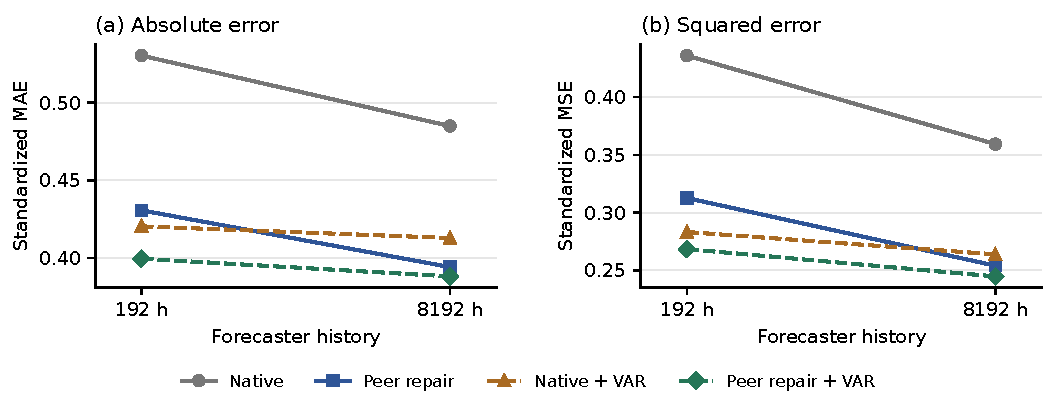
\includegraphics[width=\linewidth]{current_results/history_repair_fusion.pdf}
\caption{Component comparison on the 45 natural-outage Beijing windows. Each line retains its repair and fusion rule while changing only the history supplied to Chronos-2. The repair region and VAR filtering window remain 192 hours, and prefix-fitted parameters are unchanged. The plot reports observed station-macro errors; it does not show independent replicate uncertainty.}
\label{fig:components}
\end{figure}

At the long history, peer repair alone obtains 0.394116/0.254031, while its fixed fusion obtains 0.388053/0.244688. The repair operation already accounts for much of the natural-outage improvement, and fusion adds a smaller increment. Gaussian repair alone also performs well at 0.391787/0.252425, reducing MAE/MSE by 19.19\%/29.75\% relative to the same long native input. These comparisons separate additional historical information, target repair and statistical forecast combination. They do not attribute all of the gain to a learned decision mechanism.

Artificial outages and longer horizons produce different rankings. On artificial target outages, the primary reaches 0.631104/0.811784. Local ridge repair followed by long target-only forecasting is substantially better at 0.507640/0.542087. Relative to long native-plus-VAR, the primary has slightly lower MAE and higher MSE. At horizon 96, the primary obtains 0.809889/1.328908, while long target-only native forecasting obtains the lower MAE 0.789801 and its VAR fusion obtains the lower MSE 1.313030. The primary remains fixed in these comparisons; the stronger row in each panel is not substituted into its definition.

\subsection{Transfer of Statistical Components to HDB}

Table~\ref{tab:hdb} reports the three HDB panels without filling in an unavailable result for the peer-regression primary. Gaussian target repair and its fixed VAR fusion instantiate the available statistical components with the same fitting-only data boundary. On natural gaps, long native target-only forecasting obtains 1.178178/3.887765. Long Gaussian repair with peers obtains 1.434379/4.706353, and VAR fusion further raises MAE to 1.546516. Even the best-MAE evaluated long repair, target-only median repair at 1.263786/4.012167, remains 7.27\%/3.20\% above the native target-only control. Two additional query-mask controls retain the long native history while restricting unknown auxiliary-future attention keys along time or along both time and group dimensions. They consume no measured future inputs and are retained for their competitive results.

\begin{table}[t]
\caption{HDB component-transfer results. Long histories use all available pre-origin values up to the fixed context limit. The exact peer-regression primary is unmeasured on HDB; Gaussian rows are separately defined component variants. Bold marks the lowest displayed error.}
\label{tab:hdb}
\centering\footnotesize
\setlength{\tabcolsep}{3.3pt}
\begin{tabular}{lrrrrrr}
\toprule
 & \multicolumn{2}{c}{Natural gaps} & \multicolumn{2}{c}{Artificial outage} & \multicolumn{2}{c}{Native grid}\\
Method & MAE & MSE & MAE & MSE & MAE & MSE\\
\midrule
Native, 192 h & 1.2617 & 4.1144 & 0.6863 & 1.2566 & 0.4657 & 0.6436 \\
Native, long & 1.2006 & 3.9136 & 0.6796 & 1.3017 & 0.4488 & 0.6405 \\
Native, long, target only & \textbf{1.1782} & 3.8878 & 0.6789 & 1.3722 & 0.4521 & 0.6482 \\
VAR & 1.7269 & 4.9909 & 1.2949 & 3.1104 & 1.1826 & 2.7344 \\
Native, long + VAR & 1.4071 & 3.9467 & 0.8507 & 1.3853 & 0.7319 & 1.0201 \\
Gaussian repair, long & 1.4344 & 4.7064 & 0.9145 & 2.1494 & 0.4483 & 0.6424 \\
Gaussian repair, long + VAR & 1.5465 & 4.5873 & 1.0598 & 2.3915 & 0.7324 & 1.0205 \\
Median repair, long, target only & 1.2638 & 4.0122 & 1.2083 & 2.3544 & 0.4528 & 0.6495 \\
Median repair, long, with peers & 1.2662 & 3.9810 & 1.1726 & 2.2521 & 0.4477 & \textbf{0.6380} \\
Auxiliary-query mask, time & 1.1938 & 3.9026 & 0.6689 & 1.2575 & \textbf{0.4468} & 0.6390 \\
Auxiliary-query mask, time/group & 1.1827 & \textbf{3.8757} & 0.6709 & 1.3002 & 0.4509 & 0.6480 \\
Nine-candidate median, 192 h & 1.2435 & 4.0190 & 0.8211 & 1.6246 & 0.4727 & 0.6483 \\
Corruption-trained LoRA, 192 h & 1.2330 & 3.9595 & \textbf{0.6432} & \textbf{1.1200} & 0.4690 & 0.6497 \\
\bottomrule

\end{tabular}
\end{table}

On HDB artificial outages, corruption-trained LoRA gives 0.643229/1.120020, outperforming the 336-hour native control by 4.08\%/7.42\%. This adapted model does not exceed the strongest native control on natural gaps. On the native-grid panel, Gaussian repair without fusion is close to long native forecasting, while the VAR branch has considerably higher error. The outcome is consistent with the component-error requirement in Equation~\ref{eq:identity}; it does not identify a single cause of the cross-source difference. The HDB results constrain claims about transferring a Beijing repair-and-fusion design to other applications.

\section{Discussion}
\label{sec:discussion}

The main empirical result is a reduction in forecasting error after naturally missing PM histories when related observations, target-only statistical repair and a long model context are combined. Equal fusion adds a smaller improvement, and a Gaussian replacement for peer ridge performs nearly identically. This places the result at the level of a concrete applied forecasting procedure. Ridge regression, Gaussian conditioning and forecast averaging are established components, and the present evidence does not isolate a new statistical principle from their combination.

The application scope and primary method were chosen using repeatedly examined development data. Missing future labels restrict scoring to observed outcomes, and the event eligibility conditions exclude prolonged gaps with insufficient future support. Source, calendar period, label observability and missingness differ across the natural and artificial panels, preventing a causal attribution of their ranking differences to missingness alone. The exact primary has been evaluated on one source and one frozen backbone; the HDB component study is smaller and does not evaluate that exact procedure. Exclusion of all evaluation sources from foundation-model pretraining has not been established. Independent data with frozen eligibility and fitting rules are necessary to assess generalization of the selected procedure.

\section{Conclusion}
\label{sec:conclusion}

\method{} combines prefix-fitted peer regression, protected long-history input and fixed statistical forecast fusion. On the studied Beijing natural-outage cohort, it reduces MAE/MSE by 5.98\%/7.26\% relative to native prediction with the same long history and VAR branch. Comparable Gaussian repair, stronger controls on artificial outages and longer horizons, and unfavorable HDB component transfer delimit the result. The resulting method is fully specified and executable; its predictive advantage is currently supported for the observed natural-outage sensor cohort.
